\newpage
% \clearpage
\pagenumbering{arabic}
\setcounter{page}{17}

\section{Introdução}
\label{intro}

A segmentação de imagens assume um papel fundamental no campo de visão computacional e análise de cenas, desempenhando uma função instrumental no auxílio de atividades humanas complexas. Embora a segmentação em si não desencadeie uma ação, a sua aplicação está profundamente enraizada em diversas áreas que dependem de análise visual.

Em particular, na medicina, a segmentação de imagens tem sido uma ferramenta valiosa, possibilitando avaliações analíticas mais precisas e detalhadas \citep{Lai2015, Withey2008}. É visível, por exemplo, na radiologia, onde a segmentação é aplicada para delimitar com precisão tumores \citep{Malkanthi2017}, proporcionando informações vitais para a programação de intervenções cirúrgicas e tratamentos oncológicos. O mesmo se aplica à quantificação de volumes teciduais e ao mapeamento preciso de órgãos específicos a partir de exames de imagem \citep{Gibson2018, Schoppe2020}. Estas aplicações culminam em uma melhor compreensão da anatomia do paciente e possíveis patologias, levando a decisões de tratamento mais bem fundamentadas e precisas. A Figura \ref{intro:fig:1} demonstra situações em que a segmentação de imagens desempenha um papel imprescindível no cenário médico.

\begin{figure}[H]
    \centering
    \caption{Exemplos de aplicação da segmentação no contexto médico, representando segmentação de vasos sanguíneos, câncer de pele, câncer pulmonar e núcleos celulares, respectivamente.}
    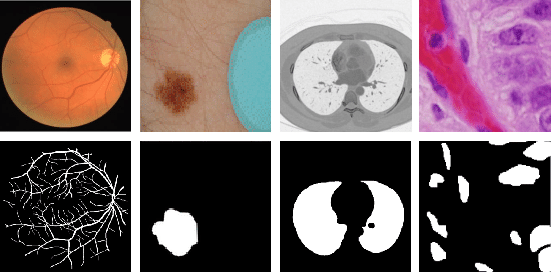
\includegraphics[width=1\linewidth]{recursos/imagens/introduction/medical-image-segmentation.png}
    \label{intro:fig:1}

    Fonte: \cite{Asadi-Aghbolaghi2020}.
\end{figure}

A segmentação de imagens e vídeos é igualmente crucial no desenvolvimento e implementação de sistemas autônomos \citep{Kaymak2019, Liu2020, Pan2020, Teichmann2018}. Nestes sistemas, que abrangem diversas áreas - da indústria ao transporte - a segmentação é frequentemente aplicada a uma variedade de tarefas essenciais.

No setor industrial, por exemplo, máquinas autônomas frequentemente dependem da segmentação para realizar tarefas de controle de qualidade. Isso envolve a análise meticulosa de imagens de produtos em linhas de montagem para identificar, por exemplo, possíveis defeitos de fabricação.

De modo similar, em sistemas de transporte autônomo, como carros completamente automatizados, a segmentação de imagens é vital para garantir a segurança e a eficácia operacional. Tais sistemas utilizam a segmentação para distinguir e identificar precisamente vários elementos em um ambiente de condução - como pedestres, placas de trânsito e sinais de trânsito, conforme desenvolvido por \cite{Lee2018} e \cite{Fleyeh2004}. Esta análise permite que o sistema reaja de maneira adequada a uma variedade de situações de condução e potenciais obstáculos \citep{Lee2018, Fleyeh2004, Pan2020}. A Figura \ref{intro:fig:2} apresenta exemplos de tais aplicações, evidenciando o papel crucial que a segmentação de imagens e vídeos desempenha em sistemas autônomos.

\begin{figure}[H]
    \centering
    \caption{Exemplos de segmentação em sistemas autônomos.}
    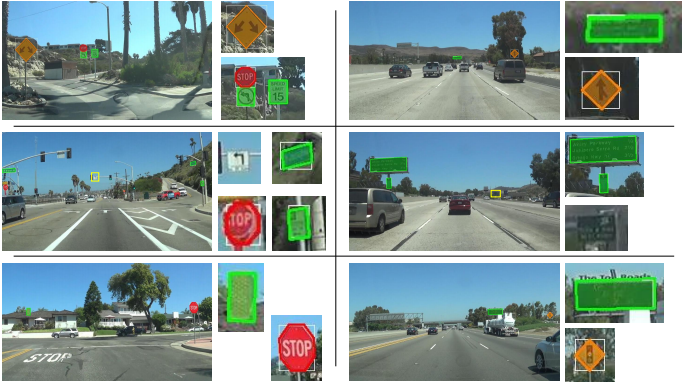
\includegraphics[width=1\linewidth]{recursos/imagens/introduction/placas.png}
    \label{intro:fig:2}

    Fonte: \cite{Lee2018}.
\end{figure}

Embora a segmentação seja um passo essencial no processo de análise de imagens, como mencionado anteriormente, ela não gera diretamente uma ação. Em vez disso, a segmentação muitas vezes faz parte de um protocolo intermediário em fluxos de trabalho que envolvem reconhecimento de imagens ou detecção de objetos.

Um exemplo distinto do papel primordial da segmentação pode ser observado no estudo conduzido por \cite{Carneiro2021}, onde é implementado o método \textit{GrabCut} \citep{rother2004grabcut} para a segmentação de imagens. \textit{GrabCut} é um método de segmentação baseado em grafos, uma abordagem bastante frequente no domínio da segmentação, como explorado por \cite{Yi2012}.

No caso do estudo de \cite{Carneiro2021}, o processo de segmentação é uma etapa prévia à crucial fase de detecção de doenças e pragas em folhas de café. Inicialmente, a segmentação por meio do \textit{GrabCut} é empregada para isolar as folhas de café na imagem. Seguidamente, os resultados desta segmentação servem como base para a detecção mais precisa de possíveis enfermidades ou infestações nessas folhas. A Figura \ref{intro:fig:3} ilustra essa aplicação.

\begin{figure}[H]
    \centering
    \caption{Segmentação feita com \textit{GrabCut}.}
    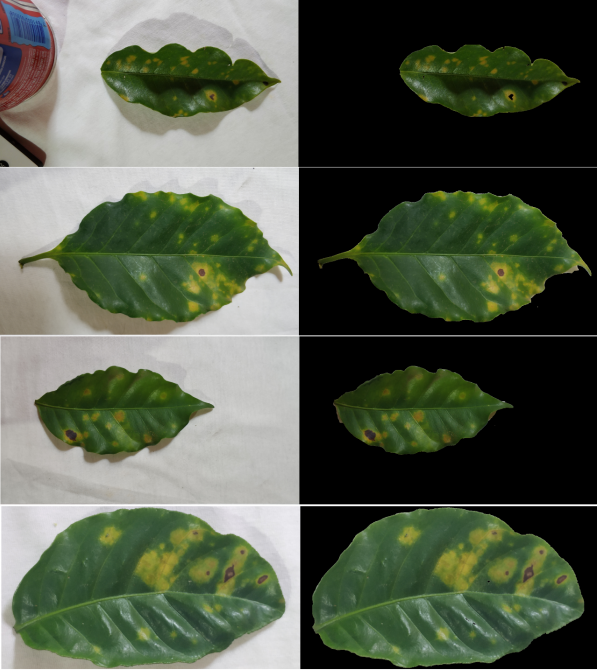
\includegraphics[height=3in]{recursos/imagens/introduction/grabcut.png}

    \label{intro:fig:3}

    Fonte: \cite{Carneiro2021}.
\end{figure}

Este estudo no domínio particular da segmentação de imagens exemplifica como tal técnica é instrumental na catalisação de processos complexos em sistemas de visão computacional. Permitindo o isolamento preciso das áreas de interesse, a segmentação promove a extração de informações mais detalhadas e relevantes a partir de imagens. Desta forma, impacta de forma significativa os resultados finais, consubstanciando-se como uma ferramenta insubstituível em uma vasta gama de aplicações práticas e estudos acadêmicos.

A segmentação de imagens revela também a sua relevância em áreas de aplicação específicas como a odontologia, que oferece várias oportunidades e desafios únicos \citep{Ghazvinian2021,Minyoung2020}. Neste domínio, há um esforço contínuo para identificar com precisão todos os componentes da cavidade bucal do paciente. Isso engloba desde o diagnóstico de patologias, como as cáries, até a avaliação do estado geral de saúde dental.

O diagnóstico na odontologia depende em grande medida da análise de imagens clínicas, e uma interpretação acurada é crucial para determinar o curso apropriado do tratamento, incluindo a necessidade de dispositivos ortodônticos \citep{Schwendicke2020}. Neste sentido, como realçado por \cite{Bansal2021, Nguyen2021} e \cite{Schwendicke2020}, as abordagens baseadas em inteligência artificial estão se mostrando soluções particularmente promissoras. Ao melhorar a precisão e a velocidade do diagnóstico, tais abordagens aprimoram o desempenho humano e consequentemente otimizam os resultados de tratamento.

Uma ilustração vívida disso é a aplicação da segmentação de imagens ao reconhecimento de dentes e cáries. Por meio da utilização de algoritmos de segmentação avançados, é possível isolar e identificar exatamente essas estruturas dentárias e patologias nas imagens, facilitando a subsequente análise e diagnóstico. A Figura \ref{intro:fig:4} apresenta alguns exemplos de aplicações da segmentação de imagens na odontologia, demonstrando o potencial desta abordagem para aprimorar a prática clínica.

\begin{figure}[H]
    \centering
    \caption{Exemplo de segmentação na área odontológica.}
    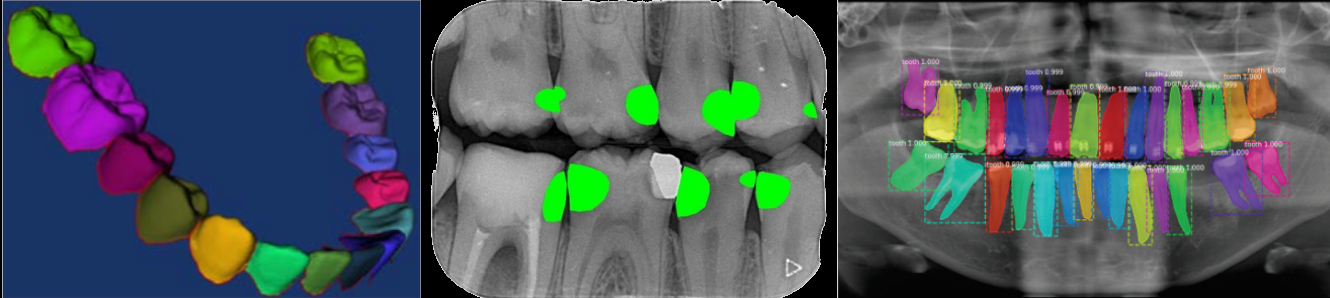
\includegraphics[width=1\linewidth]{recursos/imagens/introduction/odonto_segmentation.png}
    \label{intro:fig:4}

    Fonte: retirado e adaptado de \cite{Shuai2016,Bayrakdar2021,Gil2019}, respectivamente.
\end{figure}

Dentre as autênticas abordagens de segmentação, é significativo notar que muitos algoritmos foram desenvolvidos para responder à demanda contínua por técnicas eficazes de segmentação. Estes incluem métodos manuais sofisticados - discutidos em detalhe no Capítulo \ref{segment} - baseados em região ou limiar (Seção \ref{segment:region}), bordas (Seção \ref{segment:limit}), grafos (Seção \ref{segment:graph}), bem como algoritmos como \textit{Watershed} (Seção \ref{segment:watershed}), \textit{Livewire} (Seção \ref{segment:livewire}) e Superpixel (Seção \ref{segment:superpixel}). Também estão presentes abordagens de agrupamento (Seção \ref{segment:group}). Além disso, dada a proliferação das redes neurais, surgiram também métodos mais complexos baseados nesta técnica (Seção \ref{segment:neural}). Começa-se, então, uma incursão nos intrincados mares da temática da segmentação de imagens, com uma primeira escala nos detalhes dessas diversas técnicas de segmentação nos capítulos seguintes.

Impulsionados por melhorias contínuas em capacidades de \textit{hardware} e disponibilidade de dados, os avanços na área de aprendizado profundo têm gerado progressos notáveis, particularmente no domínio da segmentação de imagens. Esses avanços têm sido proporcionados não apenas por aprimoramentos em infraestrutura e dados, mas também pelo desenvolvimento de novos algoritmos e abordagens mais eficazes para resolver problemas complexos \citep{Szegedy2015}.

Enfatiza-se que os modelos de ponta que empregam aprendizado profundo demonstram notável capacidade de realizar combinações matriciais que destacam características específicas e podem até realizar segmentação precisa, atribuindo categorias a todos os pixels de uma imagem \citep{Minaee2021}. Isto é evidente nas redes neurais convolucionais (Capítulo \ref{cnn}) e nas técnicas de segmentação semântica (Capítulo \ref{semantic}), respectivamente.

Com as técnicas contemporâneas de segmentação, é possível lidar com dados massivos contidos nas imagens, explorando aspectos intrincados, como a escala dos objetos na cena e a dimensionalidade preservada pelos modelos. Contudo, mesmo com os avanços das técnicas de segmentação, a identificação de objetos pequenos na imagem continua a ser um desafio significativo \citep{Sang2023Small-ObjectAttention, Su2021Small-scaleFusion}. Além disso, tanto nos modelos que se utilizam de técnicas para reduzir a dimensionalidade das imagens quanto em abordagens mais recentes focadas na segmentação detalhada de imagens, um tema que se encontra pendente é em relação a avaliação crítica da adequação dos métodos comumente usados para a redução de dimensionalidade em relação à preservação espacial e consideração de visão global dos atributos.

Portanto, dentre os temas tratados, o presente projeto apresenta alguns algoritmos e \textit{frameworks} reconhecidos para segmentação, mas visa, principalmente, estudar o impacto da alteração das camadas de \textit{pooling} convencionais pelo uso do BPCAPooling em arquiteturas marcantes, como as U-Nets, avaliando suas vantagens, limitações e potenciais áreas de investigação futura que poderiam informar novos experimentos e contribuir para o progresso científico no campo da segmentação de imagens, especialmente aqueles que empregam aprendizado profundo.

\subsection{Objetivos}
\label{intro:objectives}
O objetivo geral deste trabalho consiste em propor um novo método de \textit{pooling} que, além de reduzir a dimensionalidade, preserva as informações espaciais e consideração de visão global dos atributos iniciais, visando aprimorar o detalhamento das segmentações. Tal proposta se diferencia dos métodos convencionais de \textit{pooling}, os quais não atendem a esse requisito \citep{Liu2019Multi-LevelNetworks}. Para validar essa abordagem, foram conduzidos experimentos considerando diferentes arquiteturas, desde redes convolucionais convencionais até modelos mais avançados para a segmentação semântica, buscando observar o impacto em diferentes contextos. As principais questões de pesquisa deste trabalho são:

\begin{enumerate}
    \item É possível conceber um método de \textit{pooling} que reduza a dimensionalidade, tenha uma visão global dos atributos e preserve a espacialidade?
    \item O método de \textit{pooling} proposto é capaz de substituir os métodos convencionais?
    \item Existem diferenças significativas na aplicação do método proposto entre redes convolucionais convencionais e modelos de segmentação semântica?
\end{enumerate}

A primeira questão foi explorada por meio do desenvolvimento de uma proposta de \textit{pooling} denominada \textit{Block-based Principal Component Analysis} (BPCAPooling), a qual será detalhada na Seção \ref{project:bpca}, visando abordar os desafios mencionados nessa questão específica.

O segundo item de pesquisa busca testar o método proposto em comparação com os métodos convencionalmente utilizados para a tarefa de \textit{pooling}. Esta etapa está diretamente relacionada ao terceiro ponto mencionado, o qual visa realizar esses testes em diferentes arquiteturas, desde aquelas mais antigas que introduzem conceitos de \textit{pooling} até arquiteturas mais modernas dedicadas à segmentação detalhada de imagens. Dessa forma, as contribuições desta pesquisa são:

\begin{enumerate}
    \item O desenvolvimento de um novo método de \textit{pooling};
    \item A avaliação da aplicabilidade do novo método de \textit{pooling} substituindo os métodos convencionais em redes convolucionais tradicionais;
    \item A análise da eficácia do novo método de \textit{pooling} em substituir os métodos convencionais em modelos de segmentação semântica.
\end{enumerate}


\subsection{Considerações Finais do Capítulo}
\label{intro:end}
Nos próximos capítulos, serão abordados temas relacionados à compreensão de conceitos fundamentais sobre redes neurais profundas e redes neurais convolucionais no Capítulo \ref{deep}. Em seguida, o Capítulo \ref{cnn} trará informações mais direcionadas para as redes neurais convolucionais, fundamentais para o processamento e segmentação de imagens.

O Capítulo \ref{segment} discorrerá sobre as técnicas tradicionais empregadas em atividades de segmentação. Este será seguido por uma exploração das segmentações viabilizadas pelo surgimento das redes convolucionais e de aprendizado profundo, especialmente em relação à segmentação semântica, no Capítulo \ref{semantic}.

Posteriormente, o Capítulo \ref{project} fornecerá detalhes claros sobre a metodologia proposta neste trabalho, descrevendo a estrutura do método desenvolvido e seus componentes fundamentais.

Por fim, o Capítulo \ref{results} será dedicado à apresentação dos resultados obtidos e discussões pertinentes, enquanto o Capítulo \ref{conclusion} conterá as considerações finais deste estudo.
